\documentclass{standalone}
\usepackage{tikz}
\usetikzlibrary{shapes.geometric}
\newcommand\py{1.7}
\begin{document}
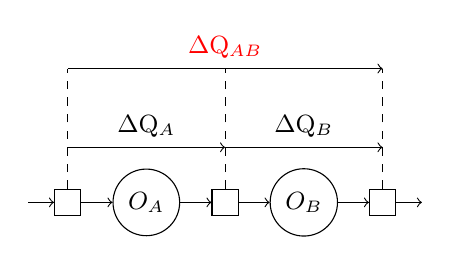
\begin{tikzpicture}[square/.style={regular polygon,regular polygon sides=4}]
\node at (0, 0) [circle, draw] (o1) {\small $O_A$}; 

\node at (2, 0) [circle, draw] (o2) {\small $O_B$};
    
    %DeltaQ marking above
    \draw [->] (-1, 0.7) -- (1,0.7) node[midway, above] {\small $\Delta$Q$_A$};
    \draw [->] (1, 0.7) -- (3,0.7) node[midway, above] {\small $\Delta$Q$_B$};
    
    \node at (-1, 0) [square, draw] (s1) {};
    \node at (1, 0) [square, draw] (e1) {};
    \node at (3, 0) [square, draw] (e2) {};

    \draw [dashed] (s1.north) -- (-1, \py);
    \draw [dashed] (e1.north) -- (1, \py);
    \draw [dashed] (e2.north) -- (3, \py);
    
    \draw [->] (-1, \py) -- (3, \py) node[midway, above, red] {\small $\Delta$Q$_{AB}$};
    %Relations events outcomes
     \draw [->] (-1.5, 0) -- (s1.west);
     \draw [->] (s1.east) -- (o1.west);

   \draw [->] (o1.east) -- (e1.west);
   \draw [->] (e1.east) -- (o2.west);
   \draw [->] (o2.east) -- (e2.west);
   \draw [->] (e2.east) -- (3.5, 0);
\end{tikzpicture}
\end{document}

